% !TEX program = pdflatex
% !TEX encoding = UTF-8 Unicode

\documentclass{scrbook}

\KOMAoptions{
    fontsize=12pt,
    paper=a4,
    %titlepage=true,
    twoside=true,
    headings=normal, % small, normal, big
    parskip=half, % full, half
    headsepline=false,
    cleardoublepage=empty,
    chapterprefix=false,
    appendixprefix=false,
    listof=totoc,
    index=totoc,
    bibliography=totoc,
    DIV=9,
    BCOR=5mm,
}

\renewcommand{\dictumwidth}{0.45\textwidth}

\usepackage{microtype}

\usepackage[utf8]{inputenc} 			    % Codificación de caracteres
\usepackage[spanish]{babel}           % Idioma

\usepackage{datetime}

\usepackage{lipsum}                   % Para incluir párrafos auxiliares de texto.

% MATEMÁTICAS
\usepackage{amsmath, amsthm, amssymb}

% TABLAS Y GRÁFICOS
\usepackage{booktabs}
\usepackage{graphicx}
  % Carpeta donde buscar los archivos de imagen por defecto
  \graphicspath{{img/}}

%\usepackage{showframe}

% ********************************************************************
% HYPERREFERENCES
% ********************************************************************
\usepackage[backref=false]{hyperref}
\hypersetup{%
	% uncomment the following line if you want to have color links
    %colorlinks=true, linktocpage=true, pdfstartpage=3, pdfstartview=FitV,%
    % uncomment the following line if you want to have black links (e.g., for printing)
    colorlinks=false, linktocpage=false, pdfborder={0 0 0}, pdfstartpage=3, pdfstartview=FitV,% 
    breaklinks=true, pdfpagemode=UseNone, pageanchor=true, pdfpagemode=UseOutlines,%
    plainpages=false, bookmarksnumbered, bookmarksopen=true, bookmarksopenlevel=1,%
    hypertexnames=true, pdfhighlight=/O,%hyperfootnotes=true,%nesting=true,%frenchlinks,%
    urlcolor=webbrown, linkcolor=RoyalBlue, citecolor=webgreen, %pagecolor=RoyalBlue,%
    %urlcolor=Black, linkcolor=Black, citecolor=Black, %pagecolor=Black,%
    pdftitle={},%
    pdfauthor={},%
    pdfsubject={},%
    pdfkeywords={},%
    pdfcreator={pdfLaTeX},%
    pdfproducer={}%
}

\usepackage{sidenotes}

\usepackage[usenames,dvipsnames]{xcolor}

% Colores
% El siguiente estilo copia el existente en Jupyter
\definecolor{backgroundcolor}{rgb}{0.97, 0.97, 0.97}     % Gris
\definecolor{keyword}{rgb}{0.22, 0.5, 0}            % Verde
\definecolor{identifier}{rgb}{0,0,0}                % Negro
\definecolor{string}{rgb}{0.75, 0.13, 0.13}         % Rojo
\definecolor{comment}{rgb}{0.75, 0.13, 0.13}
\definecolor{number}{rgb}{0.4,0.4,0.4}
\definecolor{command}{rgb}{0,0,0.5}
\definecolor{parameter}{rgb}{0.28,0.14,0.45}
\definecolor{operator}{rgb}{0.67, 0.13, 1}
\definecolor{output}{rgb}{0.03,0.4,0.03}

% Estilo secciones y subsecciones
\addtokomafont{disposition}{\fontfamily{lmdh}\selectfont}
\addtokomafont{part}{\color{brown}}
\addtokomafont{chapter}{\color{ForestGreen}}
\addtokomafont{section}{\color{red}}
\addtokomafont{subsection}{\color{blue}}

% Courier admite negrita, Computer Modern no
\renewcommand{\ttdefault}{pcr}

\usepackage{listings}
 \lstset{
   language=python,
   frame=single,
   rulecolor=\color[rgb]{0.81,0.81,0.81},
   numbers=left,
   numberstyle=\small\sffamily\color{number},
   backgroundcolor=\color{backgroundcolor},
   basicstyle=\small\ttfamily,
   commentstyle=\color{comment},
   keywordstyle=\color{keyword}\bfseries,
   stringstyle=\color{string}\itshape,
   identifierstyle=\color{identifier}
 }

\renewcommand{\lstlistingname}{Código}% Listing -> Código

% Fuente
\usepackage[T1]{fontenc}
\usepackage{accanthis}

\usepackage{subcaption}
\usepackage{wrapfig}

\usepackage{fontawesome}
\usepackage{academicons}

\usepackage[misc]{ifsym}

\usepackage{makeidx}
\makeindex

\begin{document}

\frontmatter

%! TEX root = Ejercicio 1.3 Libro

\begin{titlepage}
\begin{center}

%~\vfill %\vspace*{\fill}
\vspace*{\stretch{1}}

{\huge
  Curso Avanzado de \LaTeX: \\Libro con Ejercicios
}

\bigskip

{\large
  \textsf{David Cabezas Berrido}
}

\vfill


\includegraphics[width=60mm]{UGR.pdf}
\hfill

\includegraphics[width=60mm]{master.pdf}

\vfill

\textsc{Actualización Científica en Matemáticas}

Máster en Matemáticas \\
Universidad de Granada

\monthname \ \the\year

\vspace*{\stretch{1}}
\end{center}
\end{titlepage}

\thispagestyle{empty}
\begin{center}
    \scshape
    \lsstyle
    David Cabezas Berrido
    
    Curso Avanzado de \LaTeX: Libro con Ejercicios
\end{center}
 % portada interna

\thispagestyle{empty}

\vspace*{\fill}
\begin{flushleft}
    David Cabezas Berrido: \textit{Curso Avanzado de \LaTeX: Libro con Ejercicios,} {\scshape
    \lsstyle Estudiante del Máster en Matemáticas,} \copyright \ 2022
    
    \smallskip
    
    {\scshape
    \lsstyle Localización:} Granada, España
\end{flushleft}
\cleardoublepage

\thispagestyle{empty}

\vspace*{\fill}
\begin{flushright}

 \textit{Dedicatoria}

\end{flushright}
\vspace*{\fill}

\chapter*{Prefacio}
\addcontentsline{toc}{chapter}{Prefacio}
\thispagestyle{empty}

Prólogo del libro


\chapter*{Agradecimientos}
\addcontentsline{toc}{chapter}{Agradecimientos}
\thispagestyle{empty}

Agradecimientos del libro.

\tableofcontents

\chapter*{Introducción}
\addcontentsline{toc}{chapter}{Introducción}

Introducción del libro.

\mainmatter

\setpartpreamble[u][\textwidth]{
\begin{center}
Preámbulo primera parte
\end{center}
}
\part{Primera parte}

\chapter{Primer capítulo}

\section{Primera sección}

\begin{center}
\parbox{0.8\linewidth}{ \sffamily
Párrafo centrado y más estrecho. Sans-serif. \lipsum[75]
}
\end{center}

Como podemos ver en \cite{Euler1982}

\textbf{Definición}
Un número \emph{primo}\index{primo|textbf}\index{número!primo|textbf} es aquel número mayor o igual que $2$ que sólo es divisible por $1$ y por él mismo.

\sidenote{Esto es una nota al margen que aparece junto al contenido principal}\lipsum[1] 

\section{Segunda sección}
\lipsum[1]
\sidenote{Otra nota al margen}\lipsum[3]

\section{Tercera sección}

\lipsum[1-2] \cite{MR2009}

\subsection{Subsección}

\lipsum[1]

\part{Segunda parte}

\chapter{Segundo capítulo}

\section{Primera sección}

\dictum[Leonard Euler]{Mathematicians have tried in vain to
this day to discover some order in the
sequence of prime numbers, and we
have reasons to believe that it is a
mystery into which the human mind
will never penetrate.}

\cite{Euler1982}

\lipsum[1-3]

\part{Tercera parte: Ejercicios}

\chapter{Ejercicio 2.1}

Este ejercicio consiste en el uso y personalización del paquete \texttt{listings} para la inclusión de trozos de código en un documento \LaTeX.

\begin{lstlisting}[language=python, caption={Implementación de un perceptrón}, captionpos=b]
def dot(v, w):
    """Producto escalar de v y w """
    return sum(v_i * w_i for v_i, w_i in zip(v, w))

def funcion_activacion(x):
    """1 si la entrada es mayor o igual que 1,
    0 en otro caso."""
    return 1 if x >= 0 else 0

def perceptron(entrada, pesos):
    """1 si el perceptron se activa, 0 en otro caso"""
    return funcion_activacion(dot(entrada, pesos))
 \end{lstlisting}

\chapter{Ejercicio 2.3}

\section{Varias figuras con el paquete \texttt{subcaption}}
Como podemos ver en la Figura \ref{fig:matematicos} a Gauss, en concreto en la subfigura \ref{subfig:gauss}.

\begin{figure}[h]
    \centering
    \begin{subfigure}[t]{.24\linewidth} 
    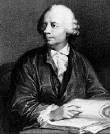
\includegraphics[height=4cm]{euler}
    \caption{Euler}\label{subfig:euler}
    \end{subfigure}
    \begin{subfigure}[t]{.24\linewidth} 
    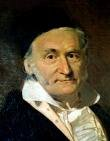
\includegraphics[height=4cm]{gauss}
    \caption{Gauss}\label{subfig:gauss}
    \end{subfigure}
    \begin{subfigure}[t]{.24\linewidth} 
    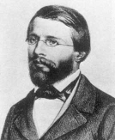
\includegraphics[height=4cm]{riemann}
    \caption{Riemann}\label{subfig:riemann}
    \end{subfigure}
    \begin{subfigure}[t]{.24\linewidth} 
    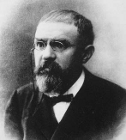
\includegraphics[height=4cm]{poincare}
    \caption{Poincare}\label{subfig:poincare}
    \end{subfigure}
    \caption{Matemáticos famosos}
    \label{fig:matematicos}
\end{figure}

Más sobre Euler en \cite{EulerWiki}.

\section{Alicia y la oruga}

La oruga y Alicia se estuvieron mirando un rato en silencio: por fin la Oruga se sacó la pipa de la boca, y se dirigió a la niña en voz lánguida y adormilada.

-¿Quién eres tú? -dijo la Oruga

No era una forma demasiado alentadora de empezar una conversación. Alicia contestó un poco intimidada:

-Apenas sé, señora, lo que soy en este momento\ldots Sí sé quién era al levantarme esta mañana, pero creo que he cambiado varias veces desde entonces.

-¿Qué quieres decir con esto? -preguntó la Oruga con severidad-. ¡A ver si te aclaras contigo misma!

\begin{wrapfigure}[16]{R}{0.30\textwidth}
  \begin{center}
    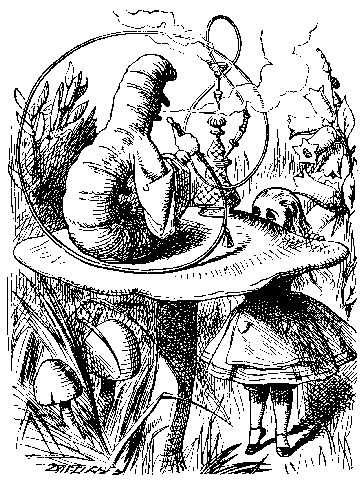
\includegraphics[width=0.30\textwidth]{oruga}
  \end{center}
  \caption{Alicia conversa con la oruga}
\end{wrapfigure}

-Temo que no puedo aclarar nada conmigo misma, señora -dijo Alicia-, porque no soy yo misma, ya lo ve.

-No veo nada -protestó la Oruga.

-Temo que no podré explicarlo con más claridad -insistió Alicia con voz amable-, porque para empezar ni siquiera lo entiendo yo misma, y eso de cambiar tantas veces de estatura en un solo día resulta bastante desconcertante.

-No resulta nada -replicó la Oruga.

-Bueno, quizás usted no haya sentido hasta ahora nada parecido -dijo Alicia-, pero cuando se convierta en crisálida, cosa que ocurrirá cualquier día, y después en mariposa, me parece que todo le parecerá un poco raro, ¿no cree?

-Ni pizca -declaró la Oruga

-Bueno,  quizá los sentimientos de usted sean distintos a los míos, porque le aseguro que a mi me parecería muy raro.

-¡A ti! -dijo la Oruga con desprecio-. ¿Quién eres tú?

Con lo cual volvían al principio de la conversación.

\appendix

\chapter{Primer apéndice}

\lipsum[66]

\setindexpreamble{Todas los números de página impresos en \textbf{negrita} hacen referencia a la
definición del término. Los números de página impresos normalmente hacen
referencia a las páginas donde dicho término es usado.\par\bigskip}

\printindex

%\nocite{*}

\setbibpreamble{Las referencias se listan por orden alfabético de acuerdo al apellido del primer autor.}

\bibliographystyle{alpha}
\bibliography{library}
\end{document}
